\section{Estilos de entrenamiento}

Las varias formas de entrenar una red se dividen en la frecuencia de la actulización de pesos, y el ajuste de sus parámetros, para ello tenemos tres formas:

\textbf{El entrenamiento en linea} en inglés \emph{batch learning} tiene esencialmente el siguiente algoritmo \ref{fig:enLinea}. Este se caracteríza en que la red es entrenada \emph{ejemplar por ejemplar}, los pesos son actualizados con cada ejemplar (más frecuencia), haciendo que durante el entrenamiento el gradiente se mueva a direcciones diferentes, por tanto es más propenso a que se llegé a dar un gradiente desvaneciente o una explosión de este. El algoritmo se da acontinuación en la fig\ref{enLines}.

\begin{figure}[H]
 \centering
 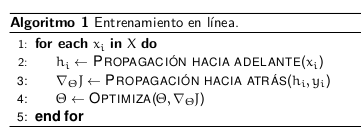
\includegraphics[scale=0.5]{../Figuras/enlinea.png}
 \caption{Algoritmo en linea.}
 \label{fig:enLinea}
\end{figure}

\textbf{El entremiento en lotes} en inglés \emph{online learning} es cuando se ajustan los pesos de la red tras haber evaluado el gradiente sobre \emph{todos los ejemplares} del entrenamiento. El cálculo del grandiente es más presiso puesto que se toman varios ejemplares en cuenta. Pero esto nos cuesta en el cómputo de la actualización de los parámetros. No es recomendable este entremiento cuando la red aún está lejos de los valores deseados. El algoritmo se da acontinuación en la fig\ref{enlotes}.

\begin{figure}[H]
 \centering
 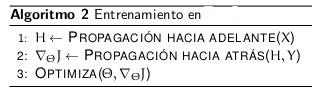
\includegraphics[scale=0.8]{../Figuras/algoritmoLotes.jpg}
 \caption{Algoritmo en lotes.}
 \label{fig:enLotes}
\end{figure}

\textbf{El entremiento en mini lotes} en este se divide el conjunto completo de entrenamiento $X$ en bloque más pequeños $X_k$ y se entrena para cada uno de ellos. Este entremiento busca un equilibrio entre el entrenamiento en linea y el entramiento por lotes, dado que no siempre vamos a tener la taza ideal de apredizaje para que el gradiente sea preciso, pero tampoco la capacidad de cómputo para entrener por lotes. 

\begin{figure}[H]
 \centering
 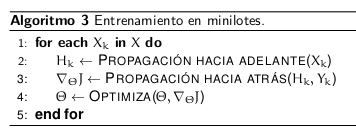
\includegraphics[scale=0.5]{../Figuras/algoritmoMiniLotes.png}
 \caption{Algoritmo en minilotes.}
 \label{fig:enLotes}
\end{figure}

Ahora veamos los pros y contra de cada entrenamiento en el entrenamiento por lotes sólo se realiza
una actualización de los pesos en cada época de entrenamiento. Para que el cálculo del gradiente del error sea fiable, se necesitará un conjunto de entrenamiento grande.
El coste computacional del cálculo del gradiente será proporcional al tamaño del conjunto de entrenamiento. Si
nuestro conjunto incluye millones de ejemplos, como suele ser habitual en big data, el coste de una iteración del algoritmo puede resultar muy costos. Dado que, se necesitarán múltiples iteraciones para conseguir que el algoritmo converja, el coste computacional del entrenamiento de la red puede ser demasiado elevado.

Así talvez no nos convenga hacer el cáculo para todos los ejemplares, entonces si tomamos una pequeña cantidad de los ejemplares tendríamos una estimación aproximada del gradiente para guiarnos. Cada vez que queramos darle un ajuste a los parámetros de nuestra red.

Ahora en el entrenamiento en linea, la estimación del gradiente, dependerá del ejemplo concreto que se escoja en cada momento, por lo que nos moveremos haciendo zigzag sobre la superficie de error. En problemas de clasificación, conviene evitar mostrarle a la red todos los ejemplos de una clase antes de pasar a los de la clase siguiente. Se recomienda mezclar bien los ejemplares para evitar cambios brusco en el cálculo del error. 

El aprendizaje online y el aprendizaje con minilotes son dos formas diferentes del gradiente descendente estocástico. El uso de minilotes suele funcionar mejor que el aprendizaje online pero si no disponemos de hardware paralelo, el aprendizaje online suele ser más rápido. Si usamos aprendizaje online, es decir $k = 1$, el uso de un único ejemplo de entrenamiento introducirá errores significativos en nuestra estimación del gradiente. En realidad, no necesitamos una estimación demasiado precisa, sólo una que nos permita movernos en una dirección adecuada, que nos facilite ir reduciendo el error de la red.
